\documentclass[9pt, a4paper]{article}

% ── Packages ──────────────────────────────────────────────────────────────────
\usepackage[top=0.60in, bottom=0.60in, left=0.75in, right=0.75in]{geometry}
\usepackage{fontspec}
\usepackage{unicode-math}
\usepackage{booktabs}
\usepackage{tabularx}
\usepackage{array}
\usepackage{graphicx}
\usepackage{enumitem}
\usepackage{hyperref}
\usepackage{xcolor}
\usepackage{titlesec}
\usepackage{parskip}
\usepackage{microtype}
\usepackage{caption}
\usepackage{placeins}

% ── Fonts ─────────────────────────────────────────────────────────────────────
\setmainfont{Arial Unicode MS}
\setmonofont{Menlo}[Scale=0.85]

% ── Colors ────────────────────────────────────────────────────────────────────
\definecolor{linkblue}{RGB}{26, 115, 232}
\definecolor{sectiongray}{RGB}{40, 40, 40}

% ── Hyperref ──────────────────────────────────────────────────────────────────
\hypersetup{colorlinks=true, linkcolor=linkblue, urlcolor=linkblue, citecolor=linkblue}

% ── Section: rule ABOVE title ─────────────────────────────────────────────────
\titleformat{\section}
  {\normalsize\bfseries\color{sectiongray}}
  {}
  {0em}
  {\vspace{2pt}\rule{\linewidth}{0.5pt}\\\vspace{3pt}}
  []
\titlespacing{\section}{0pt}{9pt}{3pt}

\titleformat{\subsection}
  {\small\bfseries}{}{0em}{}[]
\titlespacing{\subsection}{0pt}{6pt}{2pt}

% ── List spacing ──────────────────────────────────────────────────────────────
\setlist[itemize]{itemsep=1.5pt, parsep=0pt, topsep=2pt, leftmargin=1.3em}

% ── Caption ───────────────────────────────────────────────────────────────────
\captionsetup{font=scriptsize, labelfont=bf, skip=3pt}

% ── Paragraph ─────────────────────────────────────────────────────────────────
\setlength{\parskip}{3.5pt}
\setlength{\parindent}{0pt}

% ═════════════════════════════════════════════════════════════════════════════
\begin{document}
% ═════════════════════════════════════════════════════════════════════════════

% ── Header ───────────────────────────────────────────────────────────────────
{\large\bfseries State Tracking in LLMs: Models Recall the First Value but Lose the Current State}

\vspace{4pt}
\textbf{Kanak Raj} · \href{mailto:kanak8278@gmail.com}{kanak8278@gmail.com}\\
{\small \textit{Mechanistic extension of the ACL paper} ``Transformers Remember First, Forget Last: Dual-Process Interference in LLMs.''}

\vspace{2pt}\rule{\linewidth}{0.5pt}

% ── The Problem ───────────────────────────────────────────────────────────────
\section*{The Question: Can an LLM Track the State of a Variable?}

\textbf{State tracking}: a key's value is set, then updated repeatedly; we query its value at a chosen update position $k$. A stream interleaves updates to $K$ keys, each updated $N$ times. The first ($k{=}1$) and current ($k{=}N$) values are the endpoints; the real test is the interior.

The finding: models reliably return the \textbf{first} value but not the \textbf{interior or current} state --- tracking works at the edges and \textbf{collapses to the floor in between}. Sweeping $k$ (right): first-value recall is best; by $k{=}3$--$5$ accuracy is at chance and stays there. The current value is recoverable \textit{only} via the semantic anchor ``the last value'' --- asked \textit{ordinally} (``the 50th value'') it collapses too. The model holds an anchor at each end, not per-position state.

\begin{figure}[h!]
    \centering
    \begin{minipage}[b]{0.40\linewidth}
        \centering
        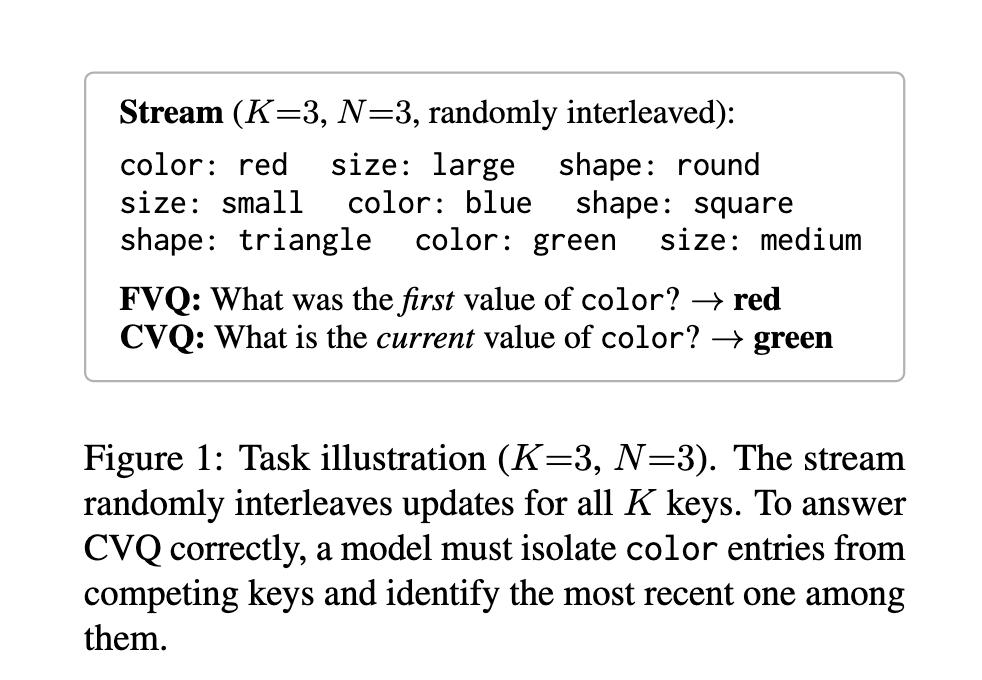
\includegraphics[width=\linewidth]{01_task.png}
    \end{minipage}\hfill
    \begin{minipage}[b]{0.585\linewidth}
        \centering
        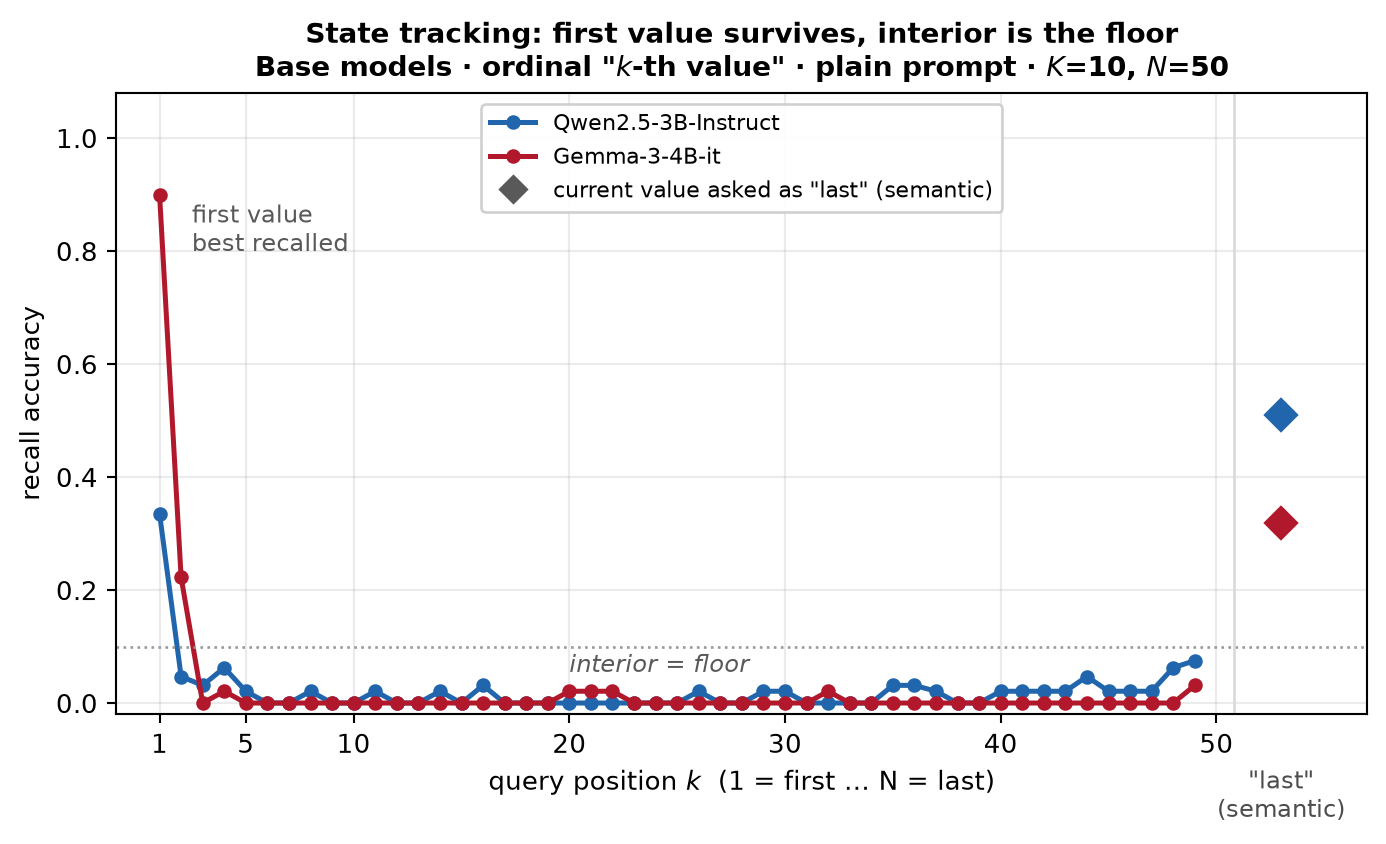
\includegraphics[width=\linewidth]{07_state_tracking_ucurve.png}
    \end{minipage}
    \caption{\textbf{Left:} the state-tracking task (caption in panel) --- updates for $K$ keys are interleaved and we query one key's value at position $k$. \textbf{Right:} per-position recall for two open-weight base models, $K{=}10$, $N{=}50$; accuracy craters after the first few positions and never recovers, and the current value is retrievable only via the semantic ``last'' anchor (diamonds).}
\end{figure}


% ── Endpoints universal ───────────────────────────────────────────────────────
\FloatBarrier
\section*{1.\;\;Even the Two Endpoints Diverge --- Universally, and Not from Context Length}

Restricting to just the two endpoints (first vs.\ current) shows the asymmetry in every model tested, proprietary and open-weight. And it is \textbf{not a context-length problem}: every failure below occurs while the prompt occupies under \textbf{3.3\%} of the model's advertised window.

\begin{figure}[h!]
    \centering
    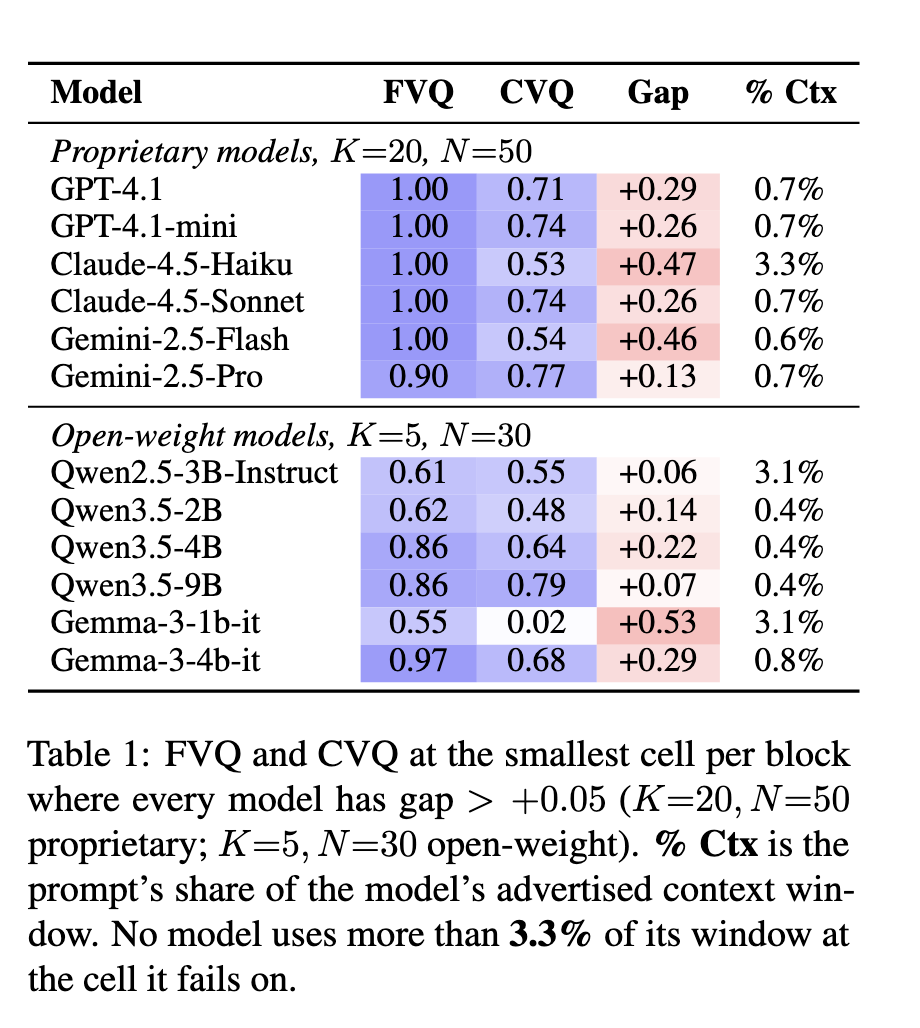
\includegraphics[width=0.33\linewidth]{02_table_fvq_cvq.png}
\end{figure}


% ── Scales with load ──────────────────────────────────────────────────────────
\FloatBarrier
\section*{2.\;\;Degrades with Interference, Not Context Length}

The current-value accuracy decays as either the number of keys $K$ or updates per key $N$ grows, while first-value recall stays pinned near $1.0$. More competing state --- not a longer prompt --- is what breaks tracking.

\begin{figure}[h!]
    \centering
    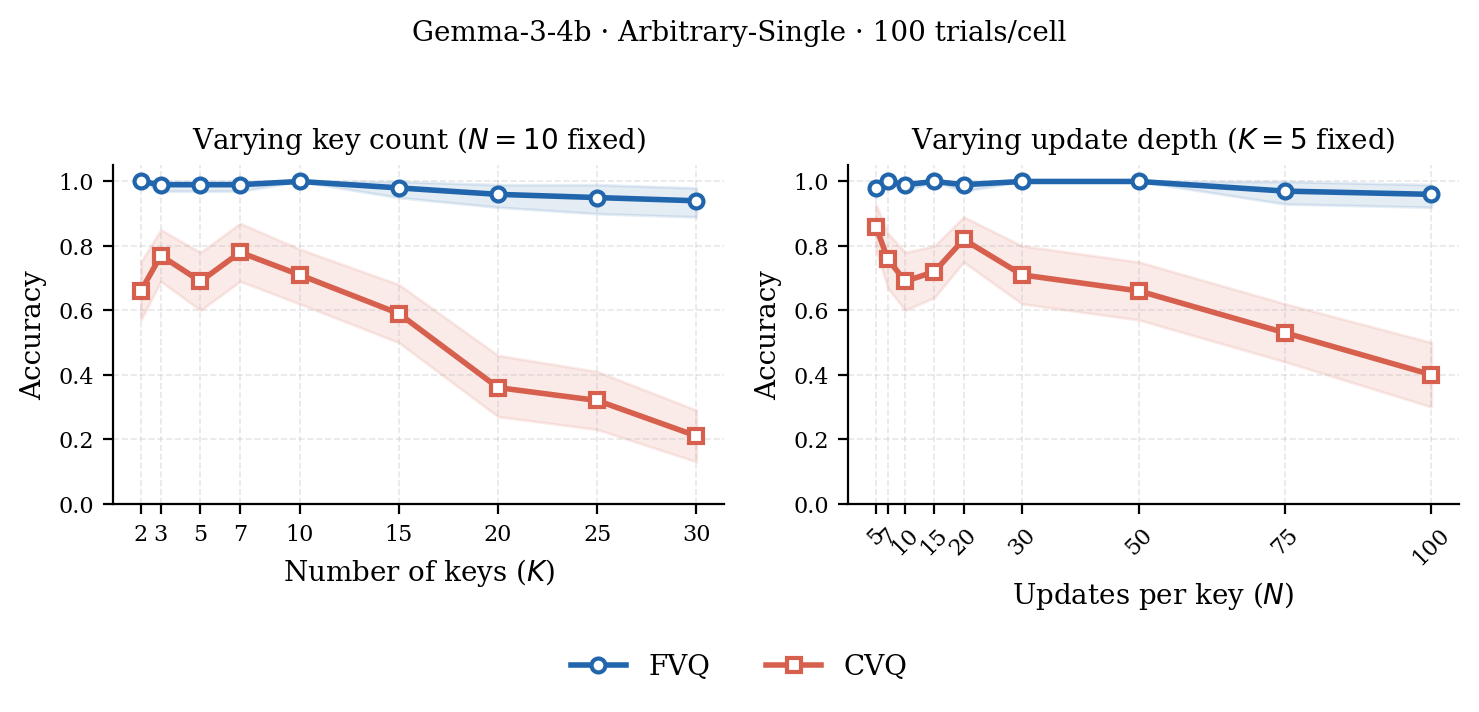
\includegraphics[width=0.68\linewidth]{03_gemma3_4b_fvq_cvq.png}
    \caption{Gemma-3-4b. First value (blue) near ceiling across both axes; current value (red) falls to $\sim$0.21 at $K{=}30$ and $\sim$0.40 at $N{=}100$.}
\end{figure}


% ── Pretraining ───────────────────────────────────────────────────────────────
\FloatBarrier
\section*{3.\;\;Present at Every Training Stage --- No Stage Causes or Cures It}

Tracking the endpoint gap across full training trajectories (SmolLM2-1.7B, SmolLM3-3B) shows it is present at the \textit{earliest} checkpoints and persists unchanged through every stage --- pretraining, SFT, mid-training, and alignment. No single stage introduces or removes it; it is not an instruction-tuning artifact.

\begin{figure}[h!]
    \centering
    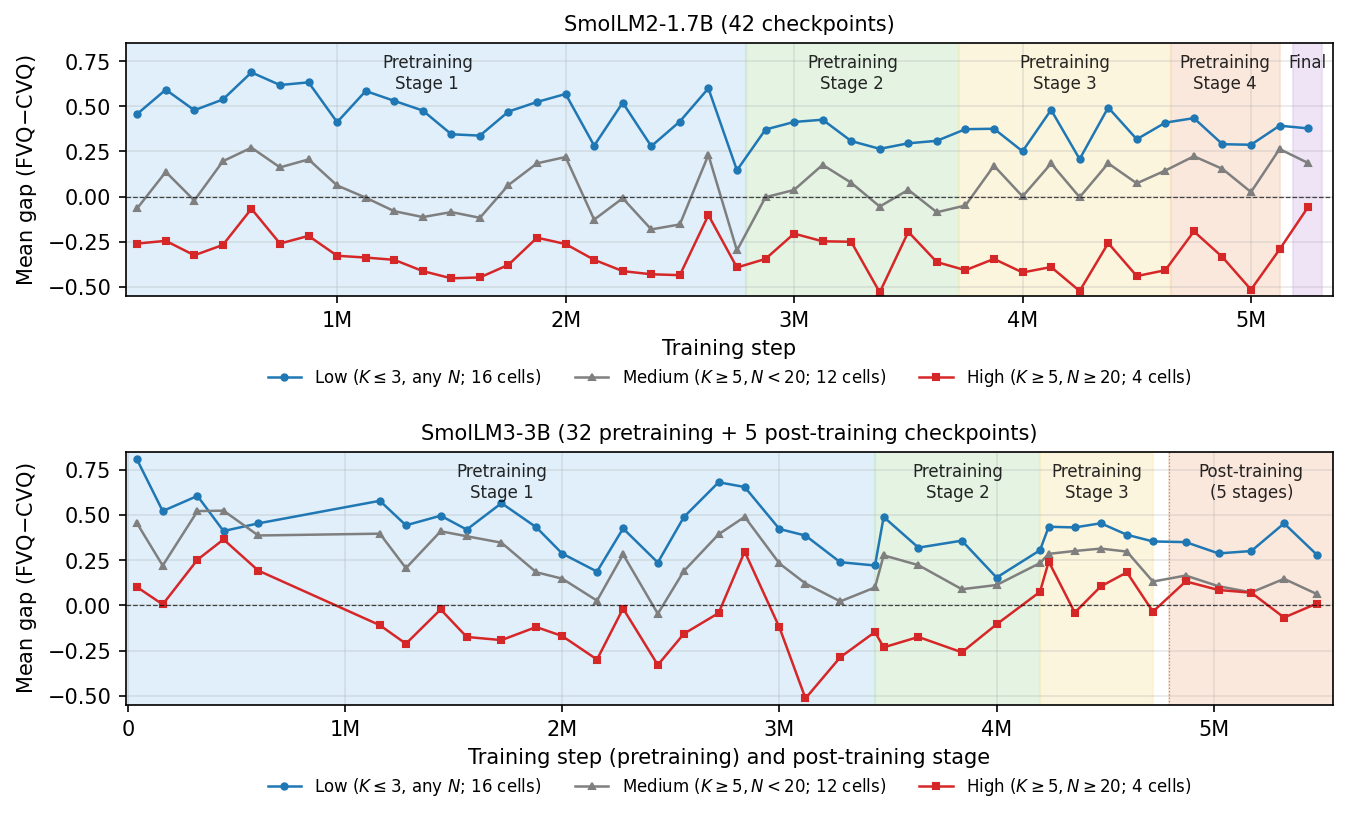
\includegraphics[width=0.62\linewidth]{04_fig3_training_dynamics.png}
    \caption{Mean first$-$current gap across 42 (SmolLM2-1.7B) and 32+5 (SmolLM3-3B) checkpoints. Positive from the first checkpoints through all pretraining and post-training stages.}
\end{figure}


% ── Mechanism ─────────────────────────────────────────────────────────────────
\FloatBarrier
\section*{4.\;\;Mechanism: the Correct State Is Computed, Then Thrown Away}

Logit lens shows \textit{where} tracking breaks. On current-value failures, the probability of the correct value rises to a peak at $\sim$85\% network depth --- the model \textit{finds} it --- then is suppressed in the final layers, outcompeted by the penultimate value. For the first value, probability rises \textbf{monotonically} to near $1.0$ with no competition. The failure is a late-layer representational collapse, consistent across architectures.

\begin{figure}[h!]
    \centering
    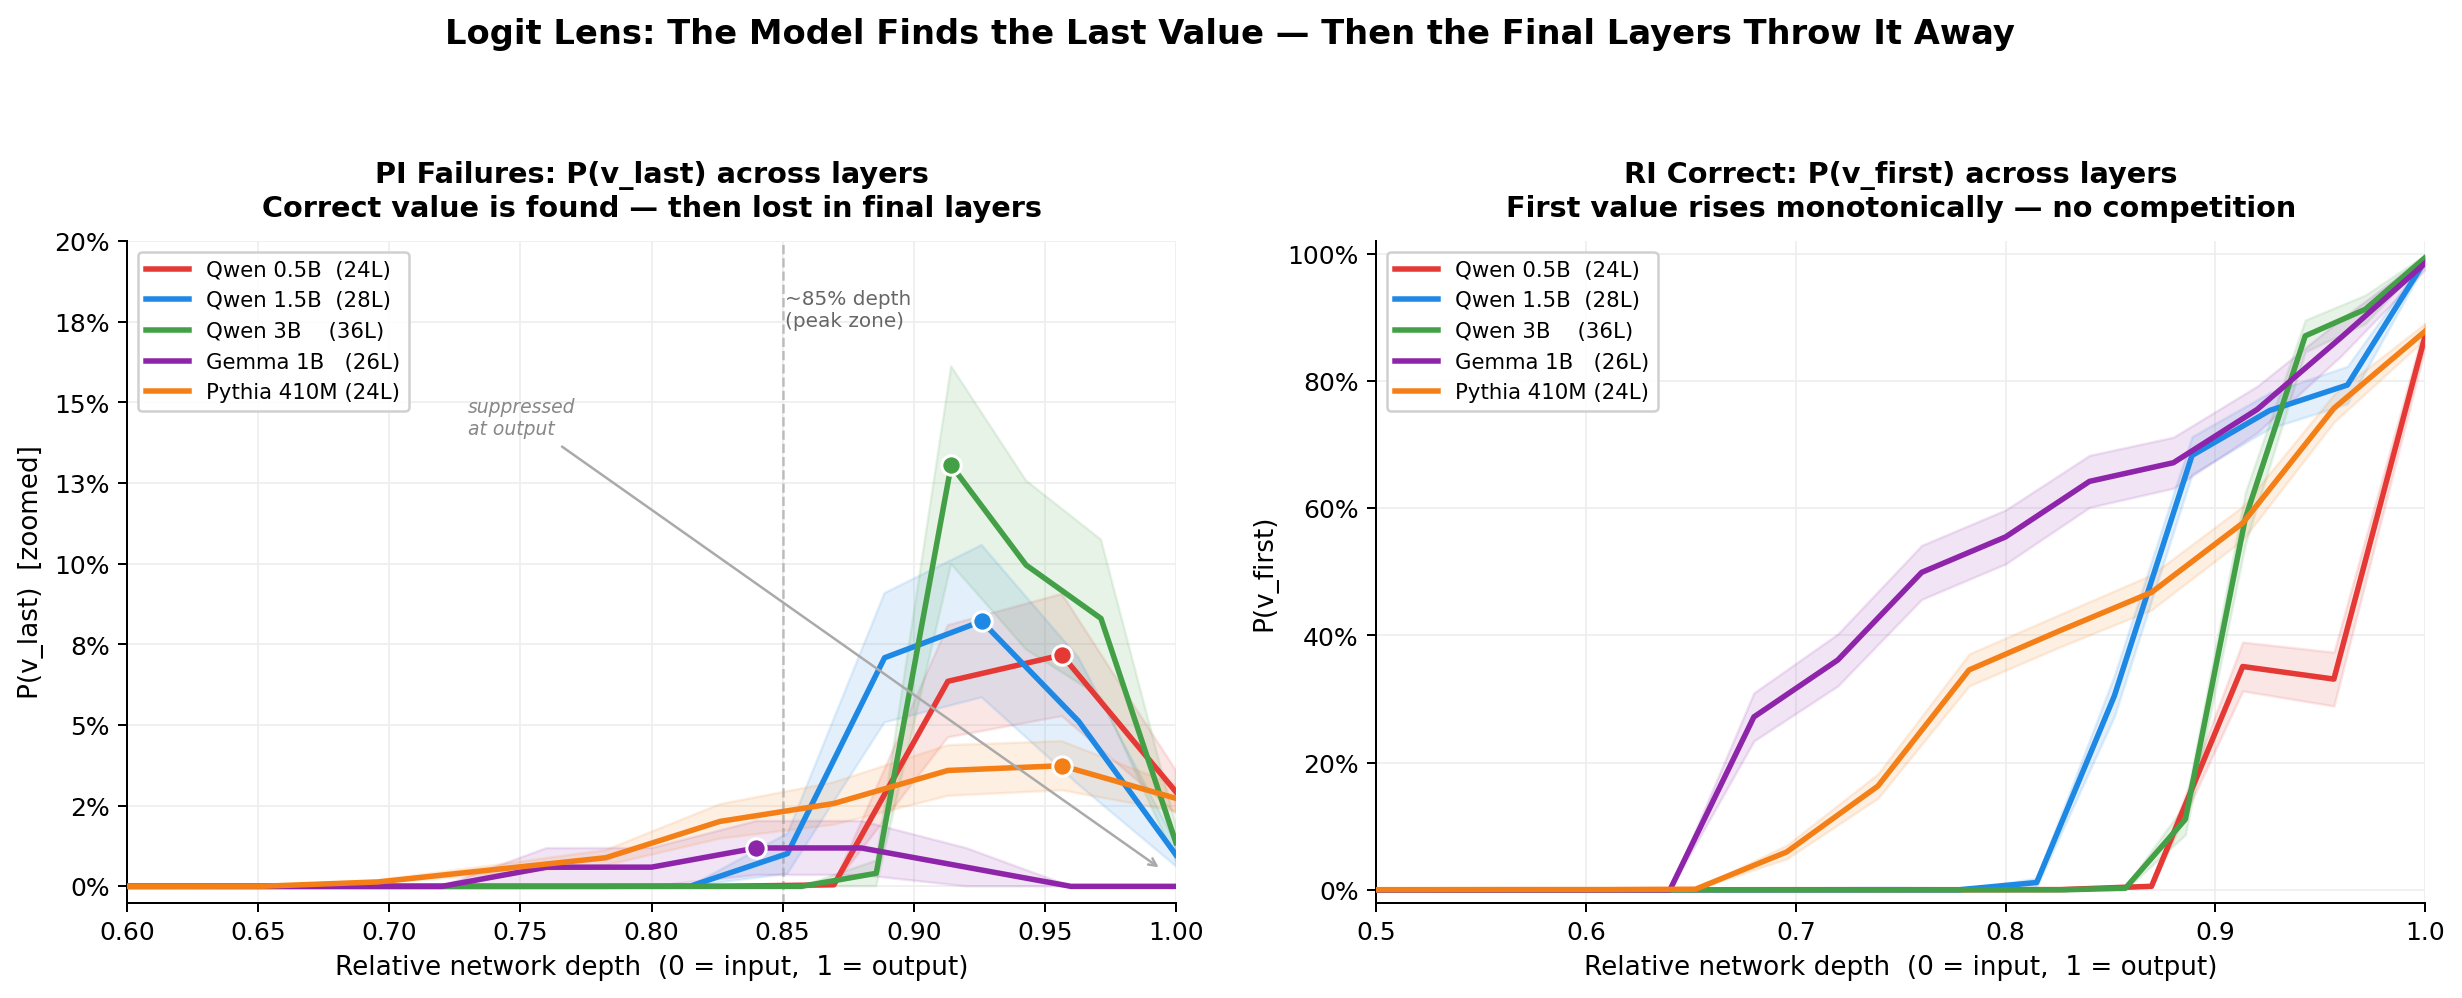
\includegraphics[width=0.55\paperwidth]{05_logit_lens.png}
    \caption{Left --- current-value failures: $P(v_\text{last})$ peaks at 81--92\% depth across 5 models, then collapses at the output. Right --- first-value correct: $P(v_\text{first})$ rises monotonically, no suppression.}
\end{figure}


% ── Naturalistic ──────────────────────────────────────────────────────────────
\FloatBarrier
\section*{5.\;\;It Survives in Natural Language, on a Frontier Model}

The effect is not a synthetic-format artifact. On naturalistic museum-visit narratives, Claude Haiku 4.5's recall decays from a primacy peak straight to the floor with \textit{no} recency bump; recency returns only through an explicit ``last'' anchor --- the same interior-floor signature.

\begin{figure}[h!]
    \centering
    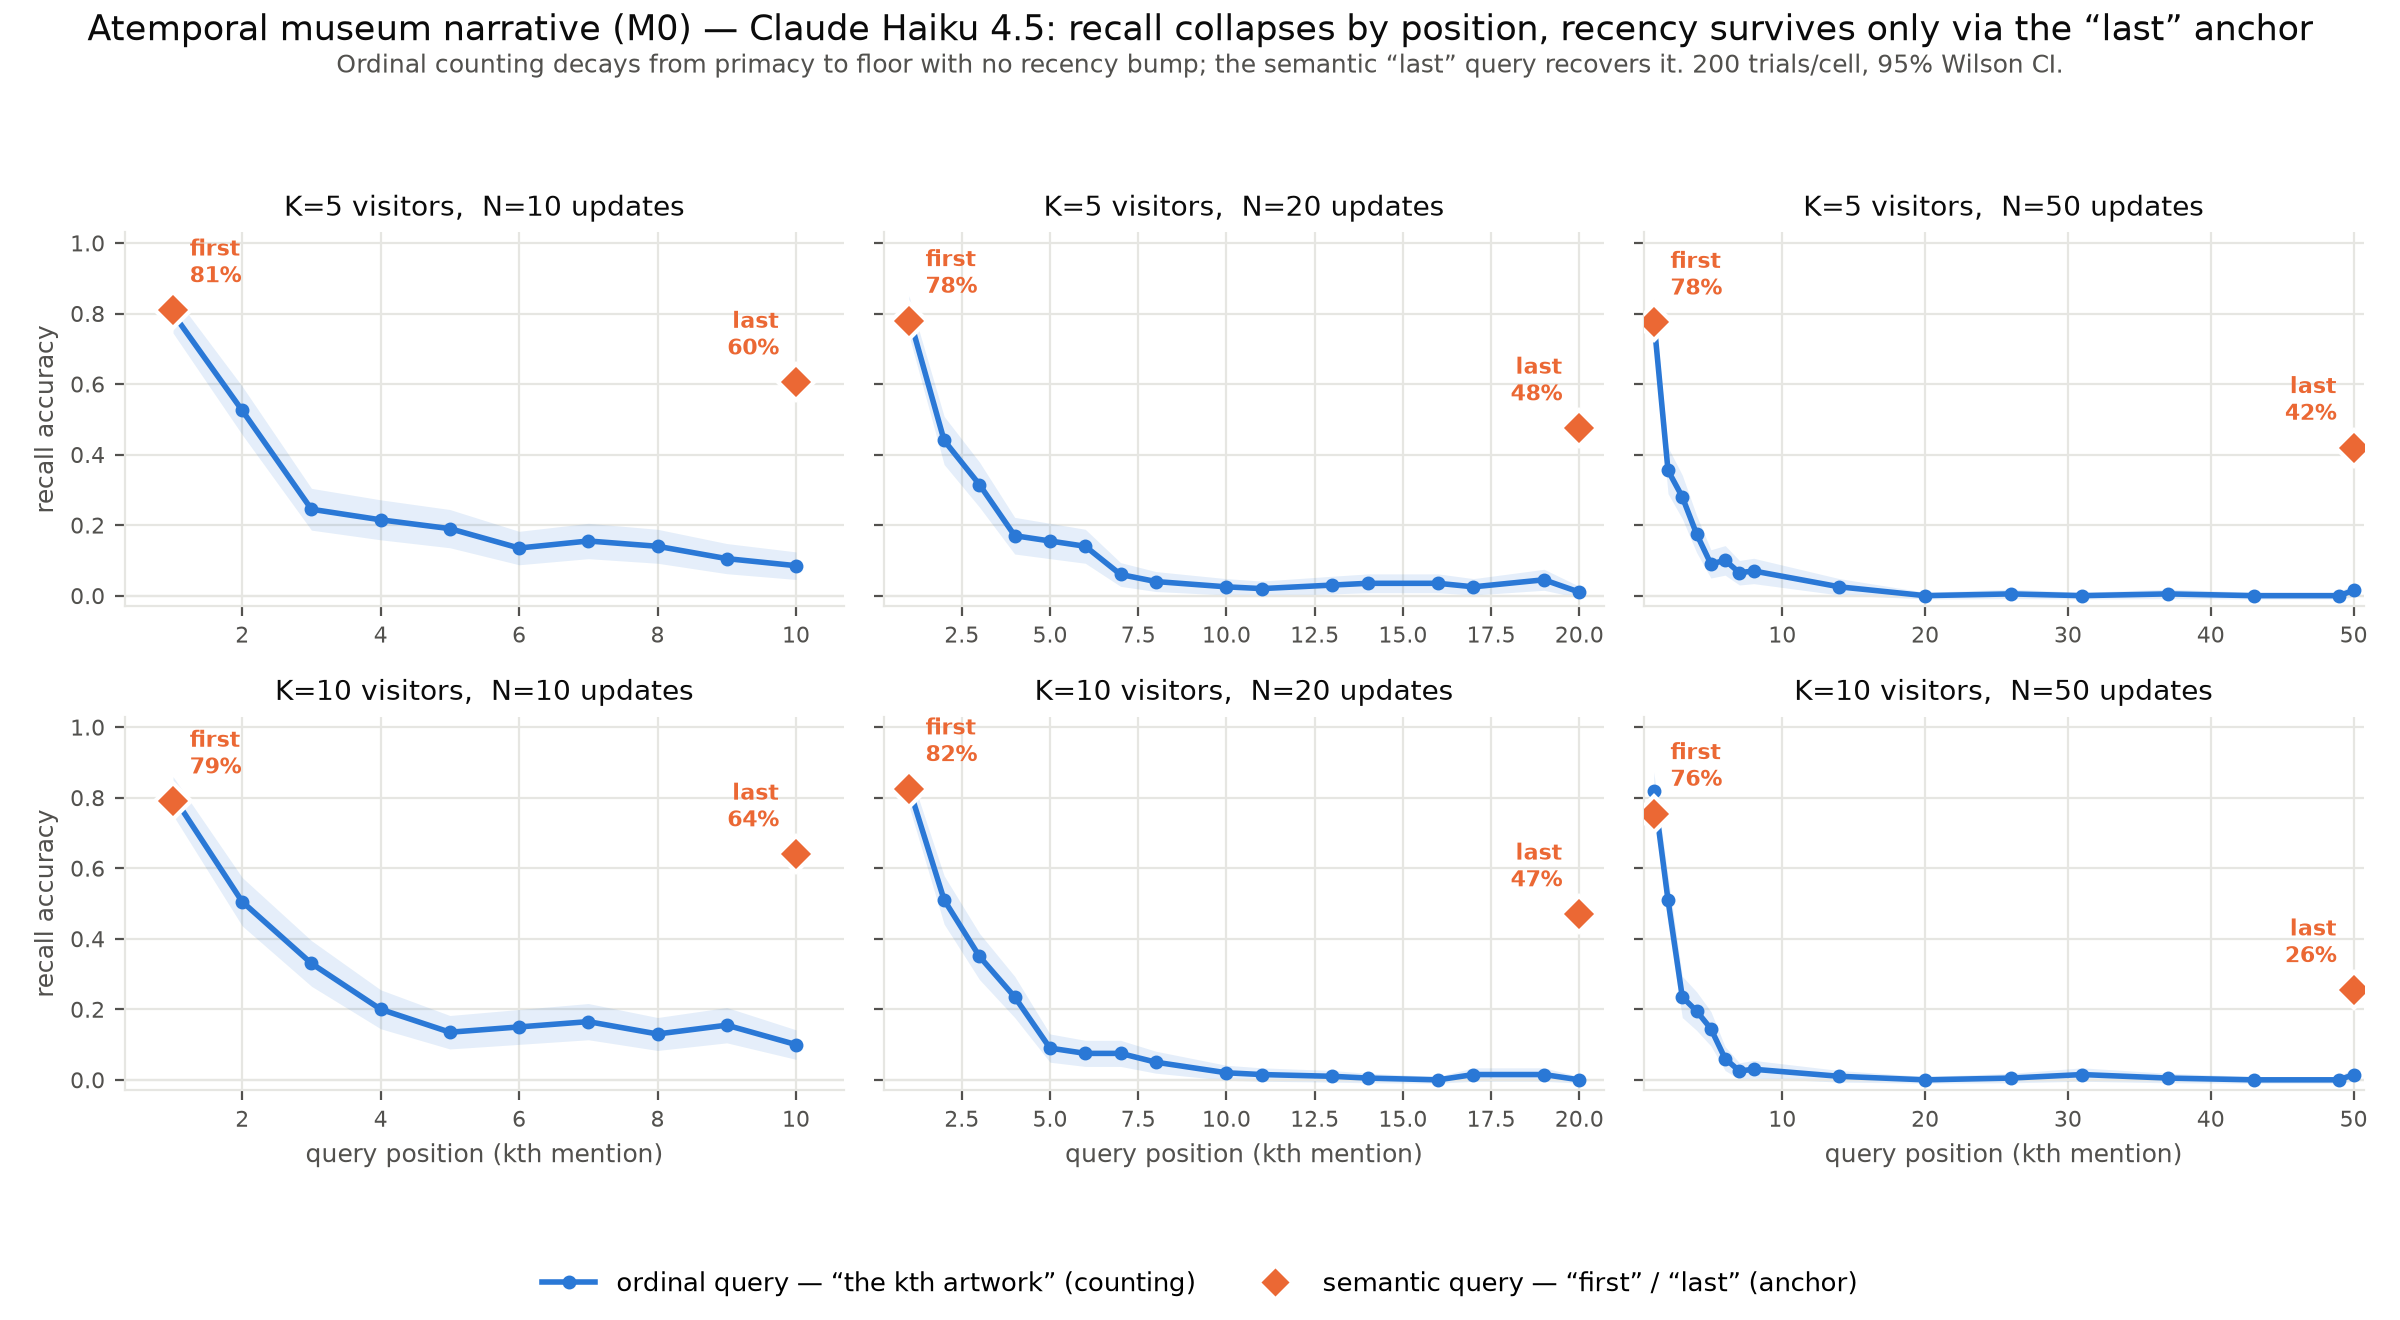
\includegraphics[width=0.55\paperwidth]{06_haiku_narrative_plain.png}
    \caption{Claude Haiku 4.5 on naturalistic narratives (200 trials/cell). Ordinal recall (blue) decays from $\sim$80\% at ``first'' to floor; only the semantic ``last'' anchor (orange) partially recovers the current state.}
\end{figure}


% ── Can we fix it ─────────────────────────────────────────────────────────────
\FloatBarrier
\section*{6.\;\;Can We Fix Interior Tracking? Format Helps; Fine-tuning Does Not Generalize}

The state \textit{is} present --- a \textbf{block} layout (grouping each key's updates) reads it back almost perfectly, lifting interior accuracy from the floor ($\sim$0.06) to $\sim$0.93--0.97. LoRA fine-tuning on the plain format also lifts the interior, but only partway, and it \textbf{decays out-of-distribution}: it learns anchors and near-training cells rather than the general ``count to the current value'' operation. Concretely, LoRA-adapted Qwen2.5-3B and Gemma-3-4B answer \textbf{first}/\textbf{last}-value queries correctly even far outside their training range, yet still \textbf{fail on mid-chain (interior) queries} at those same large cells (here ``first''/``last'' are the \textit{semantic} queries --- ``the first/last value'' --- not a numeric $k$-th position).

\begin{table}[h!]
\centering
\small
\begin{tabular}{lcccc}
\toprule
\textbf{Model (interior IVQ)} & \textbf{Base, plain} & \textbf{Base, block} & \textbf{LoRA, in-dist} & \textbf{LoRA, far-OOD} \\
\midrule
Qwen2.5-3B-Instruct & 0.06 & \textbf{0.93} & 0.55 & 0.25 \\
Gemma-3-4b-it       & 0.06 & \textbf{0.97} & 0.43 & 0.24 \\
\bottomrule
\end{tabular}
\caption{Mean interior (ordinal) accuracy. Plain-format base is at the floor; a block layout nearly solves it (the state is recoverable); LoRA lifts it in-distribution but only partially, and regresses on far-OOD $K\times N$ cells.}
\end{table}

\begin{figure}[h!]
    \centering
    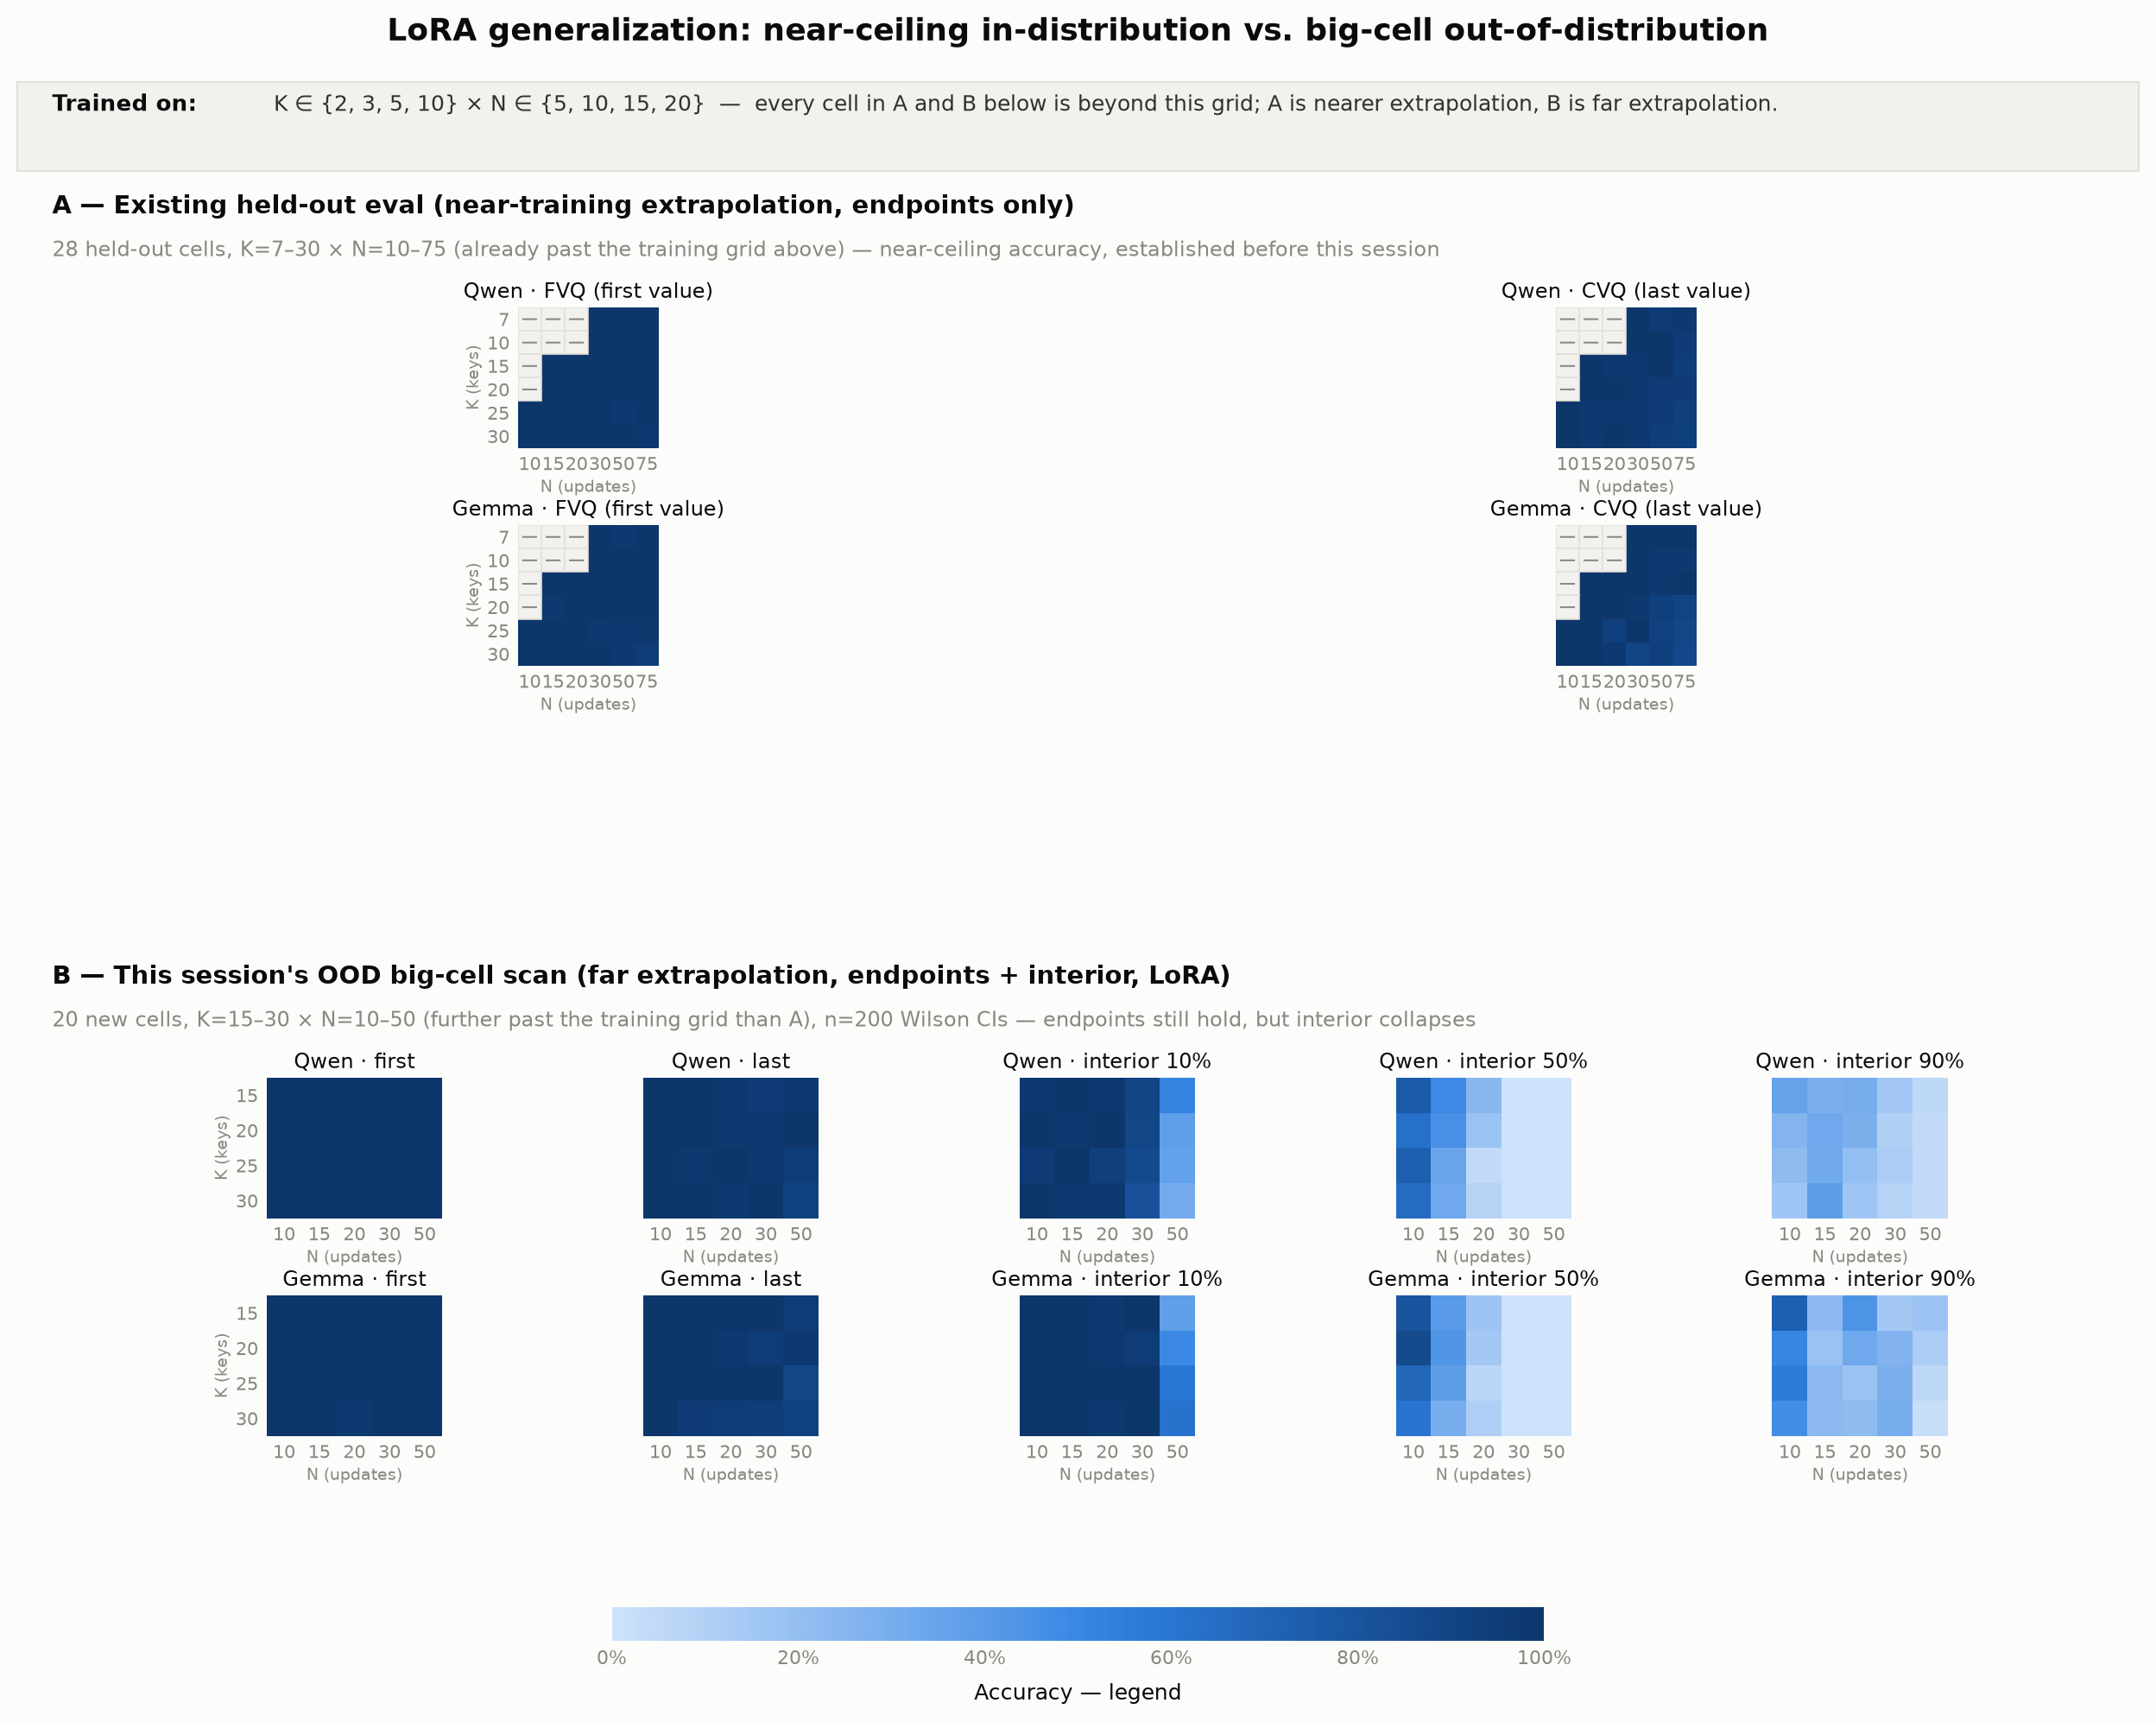
\includegraphics[width=0.55\paperwidth]{09_lora_generalization.png}
    \caption{LoRA generalization: near-ceiling in-distribution and near extrapolation (A), but far-OOD interior cells collapse while the first/current endpoints hold (B).}
\end{figure}


% ── From scratch ──────────────────────────────────────────────────────────────
\FloatBarrier
\section*{7.\;\;It Is Intrinsic to the Objective --- a From-Scratch Model Reproduces It}

A GPT-2-small trained \textit{from scratch} on the task reproduces the same structure. Within each panel accuracy is \textbf{U-shaped} --- the first and last positions are easiest, the middle hardest --- and adding keys ($K$) pushes the whole curve down. At long histories, low-to-mid $K$ stays strong while \textbf{high $K$ collapses to near-chance across every position at once}. Held-out (never-trained) cells (stars) behave like the trained ones, so this is generalization, not memorization. The bias is not inherited from web-scale data --- it emerges from the task and architecture.

\begin{figure}[h!]
    \centering
    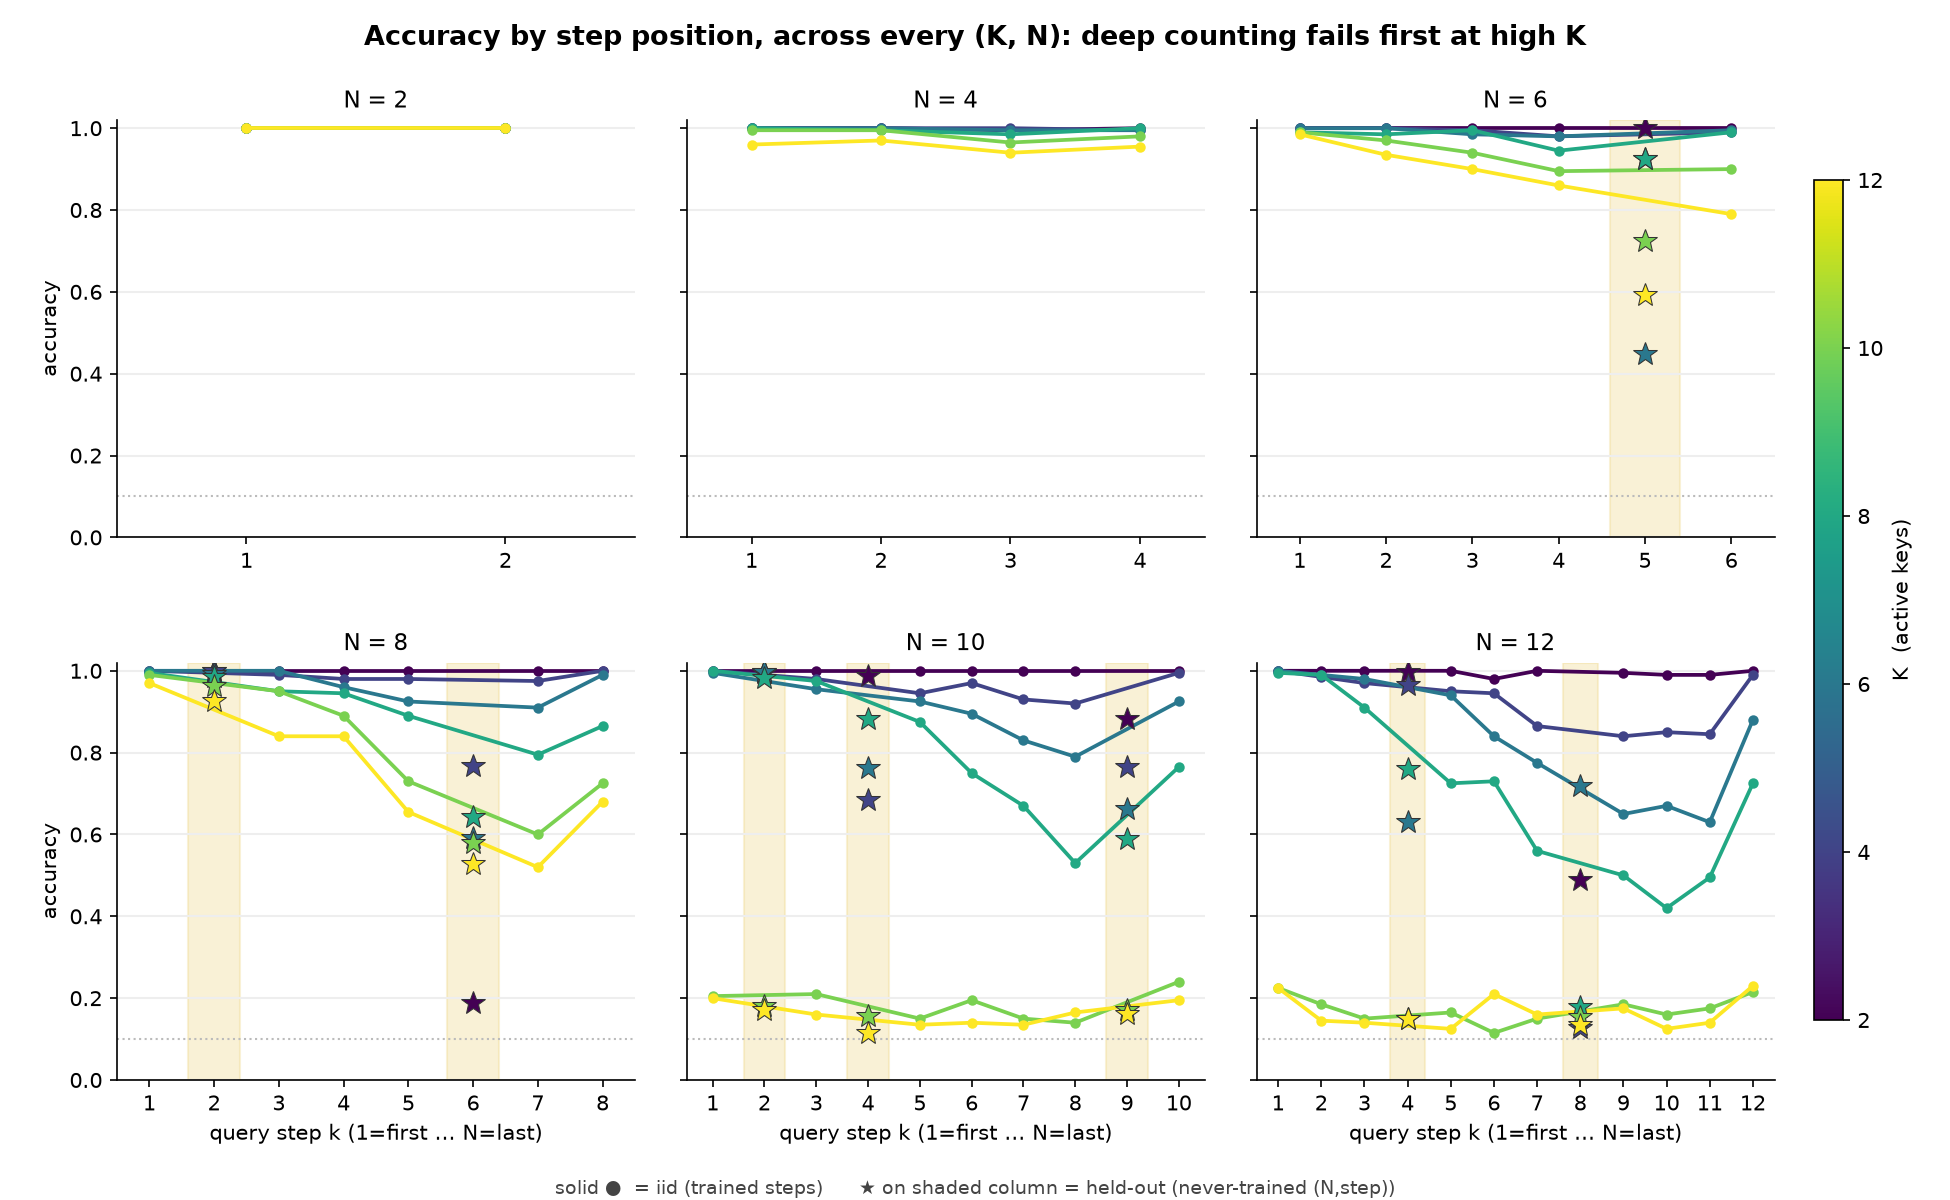
\includegraphics[width=0.55\paperwidth]{10_trained_from_scratch_ood.png}
    \caption{GPT-2-small from scratch: accuracy by query position $k$ for each $(K,N)$, colored by number of keys $K$. Within a panel the curve is U-shaped (first/last easiest, middle hardest); more keys push it down; at long $N$, high $K$ collapses across all positions. Stars mark held-out (never-trained) cells.}
\end{figure}


\vfill
\noindent\rule{\linewidth}{0.4pt}
{\scriptsize \textit{12 models (proprietary + open-weight) · 2 KV datasets + naturalistic narratives · interior position sweeps + $K\times N$ interference grids, 40--200 trials/cell · logit-lens, ablation, LoRA, and from-scratch training · SmolLM2/3 dynamics across 40+ checkpoints.}}

\end{document}
